\chapter{Introducción y nuevos objetivos}

\section{Introducción}
El número de pasajeros de avión en las últimas décadas ha aumentado exponencialmente, conllevando un aumento prácticamente similar en el tráfico aéreo. Tan sólo España tuvo el año 2012 195 millones de viajeros en la red AENA, con el aeropuerto de Madrid-Barajas 45 millones de viajeros, y el de Barcelona-El Prat 35 millones. \\
Este rápido aumento del número de aviones en el espacio aéreo, actualmente 11.000 de media por minuto, sumado a las limitaciones estructurales que tienen los aeropuertos para expenderse, ha ocasionado un importante problema de sobresaturación.
\begin{figure}[H]
	\begin{center}
		\centering
		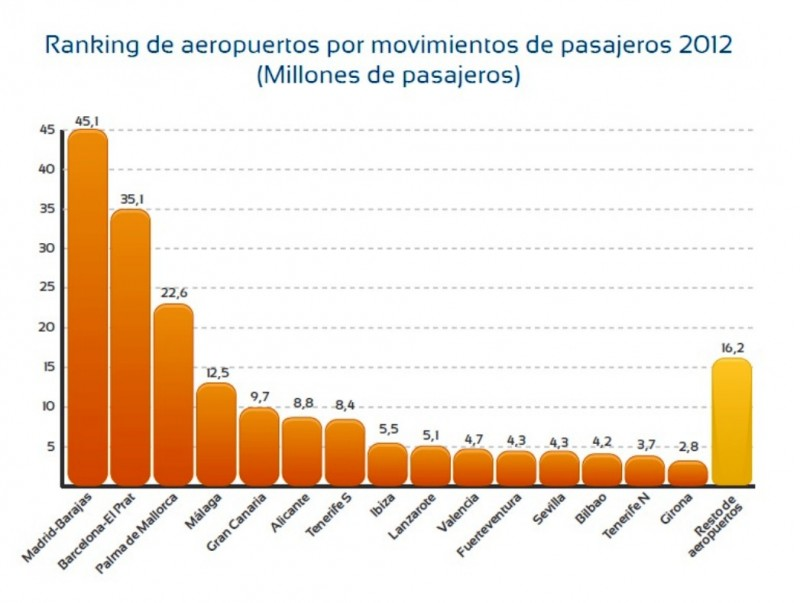
\includegraphics[width=0.7\textwidth]{./imagenes/introduccion/Ranking_de_aeropuertos_espayoles_por_pasajeros_horiz.jpg}
		\caption{Viajeros en aeropuertos españoles}
		\label{fig: Viajeros en aeropuertos españoles}
	\end{center}
\end{figure}	

Para tratar de solucionar este problema, se creó en 1988 el Central Flow management Unit, entidad dependiente de EUROCONTROL cuyo contenido es centralizar y estructurar todo el tráfico europeo, al igual que hace el Air Traffic Control System Command Center en Estados Unidos. Estas organizaciones trabajam para gestionar el tráfico aéreo a 3 niveles:
\begin{itemize}
	\item \textbf{Planificación táctica:} se realizan el mismo día, se encarga de manajar las situaciones en cada momento determinado
	\item \textbf{Planificación pre-táctica:} llevada a cabo con 2 días de antelación, se encarga de analizar el tráfico de los días previos, así como la previsión meteorológica.
	\item \textbf{Planificación estratégica: }se lleva a cabo 2 veces al año. En ella se se elaboran los planes de vuelo para cada compañía.
\end{itemize}


	
A pesar de todas las planificaciones, datos estadísticos, y mejoras en la previsión meteorológica, sigue existiendo un porcentaje importante de retrasos y cancelaciones. Según datos de EUROCONTROL, en el año 2016 un 20\% de los vuelos tuvieron un retraso mayor de 15 minutos
\begin{figure}[H]
	\begin{center}
		\centering
		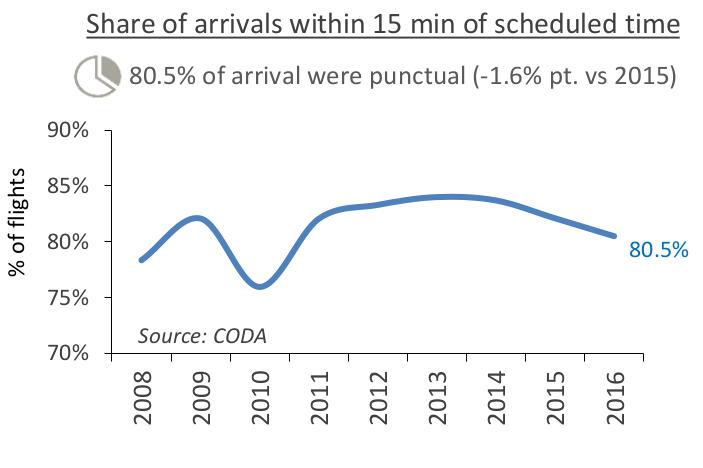
\includegraphics[width=0.7\textwidth]{./imagenes/introduccion/retrasos.png}
		\caption{Porcentaje retrasos en 2016}
		\label{fig: Porcentaje retrasos en 2016}
	\end{center}
\end{figure}

El tipo de retraso depende de la zona que estudiemos: en Estados Unidos la mayor parte de los retrasos se debe a un cuello de botella que existe en sus aeropuertos, mientras que en europa es la sobresaturación de espacios aéreos el principal problema, ya que hay un gran núnmero de aeropuertos con mucho tráfico muy cercanos unos de otros, mientras que en EEUU están más dispersos.
\begin{figure}[H]
	\begin{center}
		\centering
		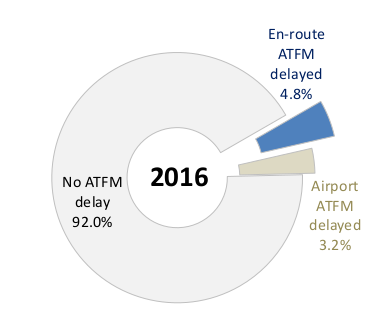
\includegraphics[width=0.7\textwidth]{./imagenes/introduccion/tiposRetrasos.png}
		\caption{Causas posibles de retraso de un vuelo}
		\label{fig: Causas posibles de retraso de un vuelo}
	\end{center}
\end{figure}

A lo largo de los últimos tiempos se han desarrollado varios modelos cuya finalidad es tratar de resolver (o l menos minimizar) el problema. Debido a que la causa más importante de los retrasos se debe al propio aeropuerto, la mayoría de los modelos se centran en tratar de resolver este cuello de botella. \\
Sin embargo, existen también modelos más complejos que también tienen en cuentya el espacio aéreo. Algunas de las estrategias que se aplican son:

\begin{enumerate}
	\item \textbf{Singe-Airport Ground-Holding Problem (SAGHP):} poco utilizada a excepción de algunos aeropuertos italianos, este modelo tiene en cuenta el número de despegues y aterrizajes que puede soportar un aeropuerto por unidad de tiempo.
	\item \textbf{Multi-Airport Ground-Holding Problem (MAGHP): }muy similar a la anterior, salvo que maneja varios aeropuertos de forma conjunta, teniendo en cuenta las relaciones entree ellos.
	\item \textbf{Air Traffic Flow Management Problem (ATFMP)}: introduce en el modelo el espacio aéreo. Como se puede ver en la figura \ref{fig: Causas posibles de retraso de un vuelo}, el porcentaje de retrasos en ruta fue mayor que el retraso en tierra. Esto se debe a que en los diferentes sectores aéreos las restricciones son menores que en los propios aeropuertos, por lo que un retraso en ruta no conlleva un retraso en otros vuelos, mientras que un retraso en un aeropuerto implica un retraso en el resto de vuelos que han de partir desde el mismo aeropuerto.
	\begin{figure}[H]
		\begin{center}
			\centering
			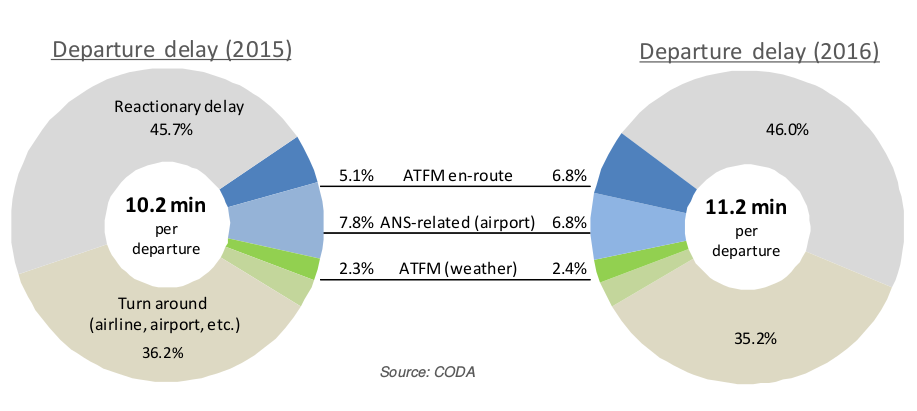
\includegraphics[width=0.7\textwidth]{./imagenes/introduccion/retrasosSalida.png}
			\caption{Comparativa retrasos 2015-2016}
			\label{fig: Comparativa retrasos 2015-2016}
		\end{center}
	\end{figure}
	\item \textbf{Air Traffic Flow Management Rerouting Problem (ATFMRP): }muy similar a ATFMP, pero añade además la posibilidad de desviar vuelos.
	\begin{figure}[H]
		\begin{center}
			\centering
			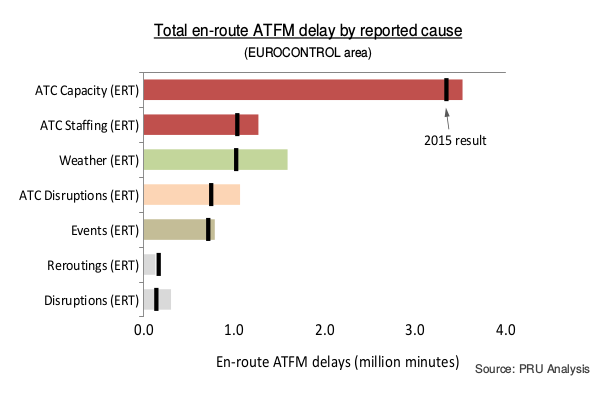
\includegraphics[width=0.7\textwidth]{./imagenes/introduccion/rerouting.png}
			\caption{Retrasos en 2016}
			\label{fig: Retrasos en 2016}
		\end{center}
	\end{figure}
	\item \textbf{Air Traffic Flow Management Rerouting with Flight Cancellation Problem (ATFMRCP): }añade la posibilidad de cancelar vuelos. Se trata de un modelo más teórico que práctico, ya que la opción de cancelar vuelos no es una opción válida para casos reales.
\end{enumerate}

\section{Versiones anteriores}
Este Trabajo Final de Grado es la continuación del trabajo que llevaron a cabo Diego Ruiz Aguado y Gonzalo Quevedo García en 2012 en sus Proyectos Finales de Carrera, los cuales se apoyaron a su vez en la Tesis Doctoral de Alba Agustín  Martín (2011).\\

A continuación se hace una breve descripción del trabajo de  Diego Ruiz Aguado y Gonzalo Quevedo García:
\begin{enumerate}
	\item Los datos del problema se encontraban en una base de datos no relacional con redundancias. El primer paso consistió en migrar esta base de datos no relacional a una base de datos MySQL relacional y bien estructurada.
	\item Para obtener los datos que necesitaba el problema, se realizó un programa en JAVA que se conectaba a la BBDD y creaba varios ficheros .txt en la que se volcaba toda la información necesaria para el posterior modelado del problema.
	\item A continuación, el programa en java leía estos ficheros .txt y creaba las estructuras de datos necesarias(árbol de rutas, vuelos, wapoints, etc).
	\item Posteriormente una subrutina en C se encargaba de definir un problema de CIPLEX con la función objetivo y las restricciones necesarias.
	\item Finalmente, se ejecutaba el problema de optimización mediante la librería CIPLEX para obtener la mejor solución del problema.
\end{enumerate}

Debido al enfoque teórico de este Trabajo de Fin de Grado, el modelo que se va a implementar se basa en el ATFMRCP, ya que permitirá cancelaciones, retrasos en aeropuertos, retrasos en ruta y desvíos. 

\section{Nuevos objetivos}
La versión anterior del problema adolecía de un importante inconveniente: no podía salir de los máximos locales, ya que el heurístico que se utilizaba para lanzar los vuelos era un algoritmo voraz. De esta forma, el resultado del problema dependía en gran medida del orden en que se intentara encontrar una solución para cada vuelo.\\

Por tanto los objetivos marcados para este Trabajo de Fin de Grado han sido los siguientes (ordenados en decreciente prioridad):
\begin{enumerate}
	\item \textbf{Mejorar heurístico: }el objetivo principal de este TFG consiste en sustituir el algoritmo voraz por un heurístico que permita al problema escapar de los máximos locales, y por tanto encontraqr una solución mejor al problema.
	\item \textbf{Desacoplar el programa de CIPLEX: }con la implementación de los nuevos heurísticos no es necesaria la librería de optimización. Se pasará de un sistema clásico de optimización (función objetivo y restricciones) a una estructura de objetos que permitan un manejo óptimo de las estructuras de datos durante la ejecución del algoritmo.
	\item \textbf{Mejorar el sistema de lectura de datos: }la versión actual del programa crea ficheros .txt en los que se vuelca toda la A2 del problema (vuelos, waypoints, routas, etc) que pueden superar las 100.000 lineas. Estos ficheros auxiliares pueden sustituirse por ficheros mucho más pequeños en los que se exporta la A2 de la base de datos, y de forma interna el problema se encarga de crear las estructuras necesarias.
	\item \textbf{Representación gráfica: }aunque estrictamente no aporta a mejorar la solución del problema, su representación gráfica puede ayudar a modelizar mejor el algoritmo, ya que permite visualizar de manera rápida y sencilla el estado del problema .
\end{enumerate}